% Options for packages loaded elsewhere
\PassOptionsToPackage{unicode}{hyperref}
\PassOptionsToPackage{hyphens}{url}
%
\documentclass[
]{article}
\usepackage{amsmath,amssymb}
\usepackage{lmodern}
\usepackage{ifxetex,ifluatex}
\ifnum 0\ifxetex 1\fi\ifluatex 1\fi=0 % if pdftex
  \usepackage[T1]{fontenc}
  \usepackage[utf8]{inputenc}
  \usepackage{textcomp} % provide euro and other symbols
\else % if luatex or xetex
  \usepackage{unicode-math}
  \defaultfontfeatures{Scale=MatchLowercase}
  \defaultfontfeatures[\rmfamily]{Ligatures=TeX,Scale=1}
\fi
% Use upquote if available, for straight quotes in verbatim environments
\IfFileExists{upquote.sty}{\usepackage{upquote}}{}
\IfFileExists{microtype.sty}{% use microtype if available
  \usepackage[]{microtype}
  \UseMicrotypeSet[protrusion]{basicmath} % disable protrusion for tt fonts
}{}
\makeatletter
\@ifundefined{KOMAClassName}{% if non-KOMA class
  \IfFileExists{parskip.sty}{%
    \usepackage{parskip}
  }{% else
    \setlength{\parindent}{0pt}
    \setlength{\parskip}{6pt plus 2pt minus 1pt}}
}{% if KOMA class
  \KOMAoptions{parskip=half}}
\makeatother
\usepackage{xcolor}
\IfFileExists{xurl.sty}{\usepackage{xurl}}{} % add URL line breaks if available
\IfFileExists{bookmark.sty}{\usepackage{bookmark}}{\usepackage{hyperref}}
\hypersetup{
  pdftitle={SME0820 - Modelos de Regressão e Aprendizado Supervisionado I - Exercício 2},
  pdfauthor={Brenda da Silva Muniz 11811603; Francisco Rosa Dias de Miranda 4402962; Heitor Carvalho Pinheiro 11833351; Mônica Amaral Novelli 11810453},
  hidelinks,
  pdfcreator={LaTeX via pandoc}}
\urlstyle{same} % disable monospaced font for URLs
\usepackage[margin=1in]{geometry}
\usepackage{color}
\usepackage{fancyvrb}
\newcommand{\VerbBar}{|}
\newcommand{\VERB}{\Verb[commandchars=\\\{\}]}
\DefineVerbatimEnvironment{Highlighting}{Verbatim}{commandchars=\\\{\}}
% Add ',fontsize=\small' for more characters per line
\usepackage{framed}
\definecolor{shadecolor}{RGB}{248,248,248}
\newenvironment{Shaded}{\begin{snugshade}}{\end{snugshade}}
\newcommand{\AlertTok}[1]{\textcolor[rgb]{0.94,0.16,0.16}{#1}}
\newcommand{\AnnotationTok}[1]{\textcolor[rgb]{0.56,0.35,0.01}{\textbf{\textit{#1}}}}
\newcommand{\AttributeTok}[1]{\textcolor[rgb]{0.77,0.63,0.00}{#1}}
\newcommand{\BaseNTok}[1]{\textcolor[rgb]{0.00,0.00,0.81}{#1}}
\newcommand{\BuiltInTok}[1]{#1}
\newcommand{\CharTok}[1]{\textcolor[rgb]{0.31,0.60,0.02}{#1}}
\newcommand{\CommentTok}[1]{\textcolor[rgb]{0.56,0.35,0.01}{\textit{#1}}}
\newcommand{\CommentVarTok}[1]{\textcolor[rgb]{0.56,0.35,0.01}{\textbf{\textit{#1}}}}
\newcommand{\ConstantTok}[1]{\textcolor[rgb]{0.00,0.00,0.00}{#1}}
\newcommand{\ControlFlowTok}[1]{\textcolor[rgb]{0.13,0.29,0.53}{\textbf{#1}}}
\newcommand{\DataTypeTok}[1]{\textcolor[rgb]{0.13,0.29,0.53}{#1}}
\newcommand{\DecValTok}[1]{\textcolor[rgb]{0.00,0.00,0.81}{#1}}
\newcommand{\DocumentationTok}[1]{\textcolor[rgb]{0.56,0.35,0.01}{\textbf{\textit{#1}}}}
\newcommand{\ErrorTok}[1]{\textcolor[rgb]{0.64,0.00,0.00}{\textbf{#1}}}
\newcommand{\ExtensionTok}[1]{#1}
\newcommand{\FloatTok}[1]{\textcolor[rgb]{0.00,0.00,0.81}{#1}}
\newcommand{\FunctionTok}[1]{\textcolor[rgb]{0.00,0.00,0.00}{#1}}
\newcommand{\ImportTok}[1]{#1}
\newcommand{\InformationTok}[1]{\textcolor[rgb]{0.56,0.35,0.01}{\textbf{\textit{#1}}}}
\newcommand{\KeywordTok}[1]{\textcolor[rgb]{0.13,0.29,0.53}{\textbf{#1}}}
\newcommand{\NormalTok}[1]{#1}
\newcommand{\OperatorTok}[1]{\textcolor[rgb]{0.81,0.36,0.00}{\textbf{#1}}}
\newcommand{\OtherTok}[1]{\textcolor[rgb]{0.56,0.35,0.01}{#1}}
\newcommand{\PreprocessorTok}[1]{\textcolor[rgb]{0.56,0.35,0.01}{\textit{#1}}}
\newcommand{\RegionMarkerTok}[1]{#1}
\newcommand{\SpecialCharTok}[1]{\textcolor[rgb]{0.00,0.00,0.00}{#1}}
\newcommand{\SpecialStringTok}[1]{\textcolor[rgb]{0.31,0.60,0.02}{#1}}
\newcommand{\StringTok}[1]{\textcolor[rgb]{0.31,0.60,0.02}{#1}}
\newcommand{\VariableTok}[1]{\textcolor[rgb]{0.00,0.00,0.00}{#1}}
\newcommand{\VerbatimStringTok}[1]{\textcolor[rgb]{0.31,0.60,0.02}{#1}}
\newcommand{\WarningTok}[1]{\textcolor[rgb]{0.56,0.35,0.01}{\textbf{\textit{#1}}}}
\usepackage{longtable,booktabs,array}
\usepackage{calc} % for calculating minipage widths
% Correct order of tables after \paragraph or \subparagraph
\usepackage{etoolbox}
\makeatletter
\patchcmd\longtable{\par}{\if@noskipsec\mbox{}\fi\par}{}{}
\makeatother
% Allow footnotes in longtable head/foot
\IfFileExists{footnotehyper.sty}{\usepackage{footnotehyper}}{\usepackage{footnote}}
\makesavenoteenv{longtable}
\usepackage{graphicx}
\makeatletter
\def\maxwidth{\ifdim\Gin@nat@width>\linewidth\linewidth\else\Gin@nat@width\fi}
\def\maxheight{\ifdim\Gin@nat@height>\textheight\textheight\else\Gin@nat@height\fi}
\makeatother
% Scale images if necessary, so that they will not overflow the page
% margins by default, and it is still possible to overwrite the defaults
% using explicit options in \includegraphics[width, height, ...]{}
\setkeys{Gin}{width=\maxwidth,height=\maxheight,keepaspectratio}
% Set default figure placement to htbp
\makeatletter
\def\fps@figure{htbp}
\makeatother
\setlength{\emergencystretch}{3em} % prevent overfull lines
\providecommand{\tightlist}{%
  \setlength{\itemsep}{0pt}\setlength{\parskip}{0pt}}
\setcounter{secnumdepth}{-\maxdimen} % remove section numbering
\ifluatex
  \usepackage{selnolig}  % disable illegal ligatures
\fi

\title{SME0820 - Modelos de Regressão e Aprendizado Supervisionado I -
Exercício 2}
\author{Brenda da Silva Muniz 11811603 \and Francisco Rosa Dias de
Miranda 4402962 \and Heitor Carvalho Pinheiro 11833351 \and Mônica
Amaral Novelli 11810453}
\date{Novembro 2021}

\begin{document}
\maketitle

\hypertarget{exercuxedcio-4}{%
\section{Exercício 4}\label{exercuxedcio-4}}

Queremos mostrar que o estimador \(F_0\) pode ser escrito na forma
\(F_0 = \frac{R^2(n-p)}{k(1-R^2)}\)

Note que podemos escrever \(SQ_{reg} = SQ_{total} R^2\). Por definição,
temos que

\[\begin{aligned}
F_0 = \frac{QM_{reg}}{QM_{res}} = \frac{\frac{SQ_{reg}}{k}}{\frac{SQ_{res}}{n-p}} = \frac{SQ_{reg}}{SQ_{res}} \frac{n-p}k = \frac{SQ_{total}\ R^2}{SQ_{total} - SQ_{reg}}  \frac{n-p}{k} = \\
\frac{SQ_{total}\ R^2}{SQ_{total} - SQ_{total}\ R^2}  \frac{n-p}{k} = 
\frac{SQ_{total}\ R^2}{SQ_{total} ( 1- R^2)}  \frac{n-p}{k} = \\
\frac{R^2(n-p)}{k (1- R^2)}.
\end{aligned}\]

Portanto, os dois são equivalentes.

\#Exercício 5

\begin{enumerate}
\def\labelenumi{\alph{enumi})}
\tightlist
\item
  Usando o exercício 4, teste a significância da regressão com
  \(\alpha = 0.05\)
\end{enumerate}

Do exercício anterior temos que: \[F_0 = \frac{R^2(n-p)}{k (1- R^2)}\]

Para \(k = 2\), \(n = 25\), \(p=k+1\) e \(R^2 = 0.90\):
\[F_0 = \frac{0.9(25-3)}{2 (1- 0.9)} = 99\]

Podemos calcular \(F_{(0.95,2,22)}\) com o seguinte comando:

\begin{Shaded}
\begin{Highlighting}[]
\CommentTok{\#calculando o valor crítico de F(0.95,2,22)}
\FunctionTok{qf}\NormalTok{(}\FloatTok{0.95}\NormalTok{,}\DecValTok{2}\NormalTok{,}\DecValTok{22}\NormalTok{)}
\end{Highlighting}
\end{Shaded}

\begin{verbatim}
## [1] 3.443357
\end{verbatim}

Logo, \(F_{(0.95,2,22)} \approx 3.443\).

Como, \(F_0 > F_{(0.95,2,22)}\), rejeitamos \(H_0\) em favor de \(H_1\)
e concluímos que o modelo testado é significante para \(\alpha = 0.05\).
Isto é, ele capta melhor a tendência dos dados se comparado ao modelo
restrito, \(y = \beta_0 + \epsilon\).

\begin{enumerate}
\def\labelenumi{\alph{enumi})}
\setcounter{enumi}{1}
\tightlist
\item
  Qual o menor valor de \(R^2\) para que o modelo seja significativo?
\end{enumerate}

Como no item anterior, vamos considerar um nível de significância
\(\alpha = 0.05\).

Sabemos que o modelo será significante se, e somente se,
\(F_0 > F_{(0.95,2,22)}\). Isso implica que:
\[\frac{R^2(n-p)}{k (1- R^2)} > 3.443\] Logo, segue que:

\[\frac{R^2(25-3)}{2 (1- R^2)} > 3.443 \\
R^2>0.2383\]

Portanto, considerando apenas dois algarismos significativos, podemos
considerar que o valor mínimo de \(R^2\) para que o modelo possa ser
considerado significativo é \(R^2 = 0.24\)

\hypertarget{exercuxedcio-11}{%
\section{Exercício 11}\label{exercuxedcio-11}}

\hypertarget{conjunto-de-dados}{%
\subsection{Conjunto de dados}\label{conjunto-de-dados}}

O dataset contém dados de um experimento para determinar \textbf{tempo},
\textbf{temperatura}, \textbf{percentual de solvatação},
\textbf{rendimento de óleo} e \textbf{carvão total} sob o
\textbf{rendimento (y)}

Significância: 97\%

Leitura dos pacotes utilizados:

Leitura do pacote de dados:

\begin{Shaded}
\begin{Highlighting}[]
\FunctionTok{library}\NormalTok{(readr)}
\NormalTok{dados }\OtherTok{\textless{}{-}} \FunctionTok{read\_csv}\NormalTok{(}\StringTok{"data{-}table{-}B5.csv"}\NormalTok{)}
\end{Highlighting}
\end{Shaded}

\begin{verbatim}
## Rows: 27 Columns: 8
\end{verbatim}

\begin{verbatim}
## -- Column specification --------------------------------------------------------
## Delimiter: ","
## dbl (8): y, x1, x2, x3, x4, x5, x6, x7
\end{verbatim}

\begin{verbatim}
## 
## i Use `spec()` to retrieve the full column specification for this data.
## i Specify the column types or set `show_col_types = FALSE` to quiet this message.
\end{verbatim}

\begin{Shaded}
\begin{Highlighting}[]
\FunctionTok{View}\NormalTok{(dados)}
\end{Highlighting}
\end{Shaded}

\begin{Shaded}
\begin{Highlighting}[]
\CommentTok{\#Renomeando as colunas}
\FunctionTok{names}\NormalTok{(dados) }\OtherTok{\textless{}{-}} \FunctionTok{c}\NormalTok{(}\StringTok{\textquotesingle{}y\textquotesingle{}}\NormalTok{, }\StringTok{\textquotesingle{}Tempo\textquotesingle{}}\NormalTok{, }\StringTok{\textquotesingle{}Temperatura\textquotesingle{}}\NormalTok{, }\StringTok{\textquotesingle{}Perc\_solvatação\textquotesingle{}}\NormalTok{, }\StringTok{\textquotesingle{}Rendimento\_Òleo\textquotesingle{}}\NormalTok{, }\StringTok{\textquotesingle{}Carvão\_Total\textquotesingle{}}\NormalTok{,}\StringTok{\textquotesingle{}x6\textquotesingle{}}\NormalTok{,}\StringTok{\textquotesingle{}x7\textquotesingle{}}\NormalTok{)}
\FunctionTok{head}\NormalTok{(dados)}
\end{Highlighting}
\end{Shaded}

\begin{verbatim}
## # A tibble: 6 x 8
##       y Tempo Temperatura Perc_solvatação Rendimento_Òleo Carvão_Total    x6
##   <dbl> <dbl>       <dbl>           <dbl>           <dbl>        <dbl> <dbl>
## 1 37.0    5.1         400            51.4            4.24        1485. 2227.
## 2 13.7   26.4         400            72.3           30.9          290.  435.
## 3 10.1   23.8         400            71.4           33.0          321.  481.
## 4  8.53  46.4         400            79.2           44.6          165.  247.
## 5 36.4    7           450            80.5           33.8         1097. 1646.
## 6 26.6   12.6         450            89.9           41.3          605.  908.
## # ... with 1 more variable: x7 <dbl>
\end{verbatim}

Para facilitar nosso trabalho em termos computacionais, estaremos
nomeando nossas variáveis e criando um data frame com as mesmas; sendo:

\begin{itemize}
\item
  \(Y:\) Rendimento total de azeite por lote de amendoim*
\item
  \(X_1:\) Tempo
\item
  \(X_2:\) Temperatura
\item
  \(X_3:\) Perc\_solvatação
\item
  \(X_4:\) Rendimento\_Òleo
\item
  \(X_5:\) Carvão\_Total
\end{itemize}

\begin{Shaded}
\begin{Highlighting}[]
\NormalTok{x1 }\OtherTok{\textless{}{-}}\NormalTok{ dados}\SpecialCharTok{$}\NormalTok{Tempo}
\NormalTok{x2 }\OtherTok{\textless{}{-}}\NormalTok{ dados}\SpecialCharTok{$}\NormalTok{Temperatura}
\NormalTok{x3 }\OtherTok{\textless{}{-}}\NormalTok{ dados}\SpecialCharTok{$}\NormalTok{Perc\_solvatação}
\NormalTok{x4 }\OtherTok{\textless{}{-}}\NormalTok{ dados}\SpecialCharTok{$}\NormalTok{Rendimento\_Òleo}
\NormalTok{x5 }\OtherTok{\textless{}{-}}\NormalTok{ dados}\SpecialCharTok{$}\NormalTok{Carvão\_Total}
\NormalTok{y }\OtherTok{\textless{}{-}}\NormalTok{ dados}\SpecialCharTok{$}\NormalTok{y}

\NormalTok{tabela01 }\OtherTok{\textless{}{-}} \FunctionTok{data.frame}\NormalTok{(}\FunctionTok{cbind}\NormalTok{(x1, x2, x3, x4, x5, y))}
\NormalTok{tabela01}
\end{Highlighting}
\end{Shaded}

\begin{verbatim}
##      x1  x2    x3    x4      x5     y
## 1   5.1 400 51.37  4.24 1484.83 36.98
## 2  26.4 400 72.33 30.87  289.94 13.74
## 3  23.8 400 71.44 33.01  320.79 10.08
## 4  46.4 400 79.15 44.61  164.76  8.53
## 5   7.0 450 80.47 33.84 1097.26 36.42
## 6  12.6 450 89.90 41.26  605.06 26.59
## 7  18.9 450 91.48 41.88  405.37 19.07
## 8  30.2 450 98.60 70.79  253.70  5.96
## 9  53.8 450 98.05 66.82  142.27 15.52
## 10  5.6 400 55.69  8.92 1362.24 56.61
## 11 15.1 400 66.29 17.98  507.65 26.72
## 12 20.3 400 58.94 17.79  377.60 20.80
## 13 48.4 400 74.74 33.94  158.05  6.99
## 14  5.8 425 63.71 11.95  130.66 45.93
## 15 11.2 425 67.14 14.73  682.59 43.09
## 16 27.9 425 77.65 34.49  274.20 15.79
## 17  5.1 450 67.22 14.48 1496.51 21.60
## 18 11.7 450 81.48 29.69  652.43 35.19
## 19 16.7 450 83.88 26.33  458.42 26.14
## 20 24.8 450 89.38 37.98  312.25  8.60
## 21 24.9 450 79.77 25.66  307.08 11.63
## 22 39.5 450 87.93 22.36  193.61  9.59
## 23 29.0 450 79.50 31.52  155.96  4.42
## 24  5.5 460 72.73 17.86 1392.08 38.89
## 25 11.5 450 77.88 25.20  663.09 11.19
## 26  5.2 470 75.50  8.66 1464.11 75.62
## 27 10.6 470 83.15 22.39  720.07 36.03
\end{verbatim}

Devido à complexidade das fórmulas envolvidas para realizarmos uma
regressão linear múltima, utilizaremos uma abordagem matricial. Desse
modo, poderemos escrever

\$y\_i = \beta\_0 + \beta\emph{1 x}\{1i\} + \beta\emph{2 x}\{2i\} +
\ldots{} + \beta\emph{k x}\{ki\} + \varepsilon\_i, i = 1, \ldots, 5. \$

como:

\(y_1 = \beta_0 + \beta_1 x_{11} + \beta_2 x_{21} + ... + \beta_k x_{k1} + \varepsilon_1\)
\(y_2 = \beta_0 + \beta_1 x_{12} + \beta_2 x_{22} + ... + \beta_k x_{k2} + \varepsilon_2\)
\(y_3 = \beta_0 + \beta_1 x_{13} + \beta_2 x_{23} + ... + \beta_k x_{k3} + \varepsilon_3\)
\(y_4 = \beta_0 + \beta_1 x_{14} + \beta_2 x_{24} + ... + \beta_k x_{k4} + \varepsilon_4\)
\(y_5 = \beta_0 + \beta_1 x_{15} + \beta_2 x_{25} + ... + \beta_k x_{k5} + \varepsilon_5\)

Assim, alocamos essas equações em dois vetores colunas (5x1), fazendo:

\begin{Shaded}
\begin{Highlighting}[]
\NormalTok{n }\OtherTok{\textless{}{-}} \FunctionTok{length}\NormalTok{(dados}\SpecialCharTok{$}\NormalTok{y)}
\NormalTok{X }\OtherTok{\textless{}{-}} \FunctionTok{matrix}\NormalTok{(}\FunctionTok{c}\NormalTok{(}\FunctionTok{rep}\NormalTok{(}\DecValTok{1}\NormalTok{,n), x1, x2, x3, x4, x5), }\AttributeTok{ncol =} \DecValTok{6}\NormalTok{, }\AttributeTok{nrow =}\NormalTok{ n, }\AttributeTok{byrow =} \ConstantTok{FALSE}\NormalTok{)}
\NormalTok{Y }\OtherTok{\textless{}{-}} \FunctionTok{matrix}\NormalTok{(y, }\AttributeTok{ncol =} \DecValTok{1}\NormalTok{, }\AttributeTok{nrow =}\NormalTok{ n)}
\NormalTok{k }\OtherTok{\textless{}{-}} \FunctionTok{ncol}\NormalTok{(X) }\SpecialCharTok{{-}}\DecValTok{1}
\NormalTok{p }\OtherTok{\textless{}{-}}\NormalTok{ k }\SpecialCharTok{+} \DecValTok{1}
\end{Highlighting}
\end{Shaded}

**

\begin{Shaded}
\begin{Highlighting}[]
\CommentTok{\#Definindo os betas do modelo de regressão múltipla}

\NormalTok{betas }\OtherTok{\textless{}{-}} \FunctionTok{solve}\NormalTok{(}\FunctionTok{t}\NormalTok{(X)}\SpecialCharTok{\%*\%}\NormalTok{X)}\SpecialCharTok{\%*\%}\FunctionTok{t}\NormalTok{(X)}\SpecialCharTok{\%*\%}\NormalTok{Y}

\CommentTok{\#Definindo a matrix C\_jj}

\NormalTok{C\_jj }\OtherTok{=} \FunctionTok{solve}\NormalTok{(}\FunctionTok{t}\NormalTok{(X)}\SpecialCharTok{\%*\%}\NormalTok{X)}

\CommentTok{\#Definindo uma matrix para os betas}

\NormalTok{betas }\OtherTok{\textless{}{-}} \FunctionTok{matrix}\NormalTok{(}\AttributeTok{data =}\NormalTok{ betas, }\AttributeTok{nrow =} \FunctionTok{length}\NormalTok{(betas), }\AttributeTok{ncol =} \DecValTok{1}\NormalTok{, }\AttributeTok{byrow =} \ConstantTok{FALSE}\NormalTok{)}
\FunctionTok{rownames}\NormalTok{(betas) }\OtherTok{\textless{}{-}} \FunctionTok{c}\NormalTok{(}\StringTok{"beta0"}\NormalTok{, }\StringTok{"beta1"}\NormalTok{,}\StringTok{"beta2"}\NormalTok{,}\StringTok{"beta3"}\NormalTok{,}\StringTok{"beta4"}\NormalTok{,}\StringTok{"beta5"}\NormalTok{)}
\NormalTok{betas}
\end{Highlighting}
\end{Shaded}

\begin{verbatim}
##              [,1]
## beta0 30.59319595
## beta1 -0.38612042
## beta2 -0.04556211
## beta3  0.31074404
## beta4 -0.37167815
## beta5  0.01409776
\end{verbatim}

Abaixo, estaremos conferindo com os valores dos betas calculados pelo
método lm. É importante ressaltar que não chamaremos o data frame do
conjunto de dados completo - visto que esse conta com as variáveis
\(x_6\) e \(x_7\) que não serão consideradas nessa análise de regressão
-, e sim a tabela com as variáveis de \(x_1\) até \(x_5\).

\begin{Shaded}
\begin{Highlighting}[]
\CommentTok{\#Modelo do R}
\FunctionTok{lm}\NormalTok{(}\AttributeTok{formula =}\NormalTok{ y }\SpecialCharTok{\textasciitilde{}}\NormalTok{., }\AttributeTok{data =}\NormalTok{ tabela01)}
\end{Highlighting}
\end{Shaded}

\begin{verbatim}
## 
## Call:
## lm(formula = y ~ ., data = tabela01)
## 
## Coefficients:
## (Intercept)           x1           x2           x3           x4           x5  
##    30.59320     -0.38612     -0.04556      0.31074     -0.37168      0.01410
\end{verbatim}

Segue abaixo a equação para o modelo determinado:

\(y= 30.59320 - 0.38612x1 - 0.04556x2 + 0.31074x3 - 0.37168x4 + 0.01410x5\)

\hypertarget{teste-de-significancia-da-regressuxe3o}{%
\subsection{Teste de significancia da
Regressão}\label{teste-de-significancia-da-regressuxe3o}}

A estimação de \(\sigma^2\) é necessária para o seguimento do teste.
Sendo assim, fazemos:

\(SQ_{res}=\boldsymbol{Y}^{T}\boldsymbol{Y}-\widehat{\boldsymbol{\beta}}^{T}\boldsymbol{X}^{T}\boldsymbol{Y}\)

\begin{Shaded}
\begin{Highlighting}[]
\NormalTok{SQRes }\OtherTok{\textless{}{-}}\NormalTok{ (}\FunctionTok{t}\NormalTok{(Y)}\SpecialCharTok{\%*\%}\NormalTok{Y)}\SpecialCharTok{{-}}\NormalTok{(}\FunctionTok{t}\NormalTok{(betas)}\SpecialCharTok{\%*\%}\FunctionTok{t}\NormalTok{(X)}\SpecialCharTok{\%*\%}\NormalTok{Y)}
\NormalTok{SQRes}
\end{Highlighting}
\end{Shaded}

\begin{verbatim}
##          [,1]
## [1,] 3222.907
\end{verbatim}

Logo, \(\widehat{\sigma}^2=\dfrac{SQres}{n-p}\).

\begin{Shaded}
\begin{Highlighting}[]
\NormalTok{p }\OtherTok{\textless{}{-}} \FunctionTok{ncol}\NormalTok{(X)}

\CommentTok{\#estimando o sigma\^{}2}

\NormalTok{sigma2 }\OtherTok{\textless{}{-}}\NormalTok{ SQRes}\SpecialCharTok{/}\NormalTok{(n}\SpecialCharTok{{-}}\NormalTok{p)}
\NormalTok{sigma2}
\end{Highlighting}
\end{Shaded}

\begin{verbatim}
##          [,1]
## [1,] 153.4718
\end{verbatim}

\hypertarget{anova}{%
\subsection{ANOVA}\label{anova}}

Agora que ajustamos um modelo inicial, é necessário que verifiquemos se
ele é adequado em explicar a variabilidade de nossa amostra. Vamos
assumir que \(\xi\sim N_n(0,\sigma^2I)\). Precisamos agora verificar
nossa suposição graficamente:

\begin{Shaded}
\begin{Highlighting}[]
\CommentTok{\# Obtendo uma estimativa para Y a partir do modelo ajustado}
\NormalTok{Y\_est }\OtherTok{\textless{}{-}}\NormalTok{ X}\SpecialCharTok{\%*\%}\NormalTok{betas}

\CommentTok{\# Cálculo dos resíduos}
\NormalTok{res }\OtherTok{\textless{}{-}}\NormalTok{ Y }\SpecialCharTok{{-}}\NormalTok{ Y\_est}
\end{Highlighting}
\end{Shaded}

\begin{Shaded}
\begin{Highlighting}[]
\NormalTok{p }\OtherTok{\textless{}{-}} \FunctionTok{ggplot}\NormalTok{(}\FunctionTok{tibble}\NormalTok{(res), }\FunctionTok{aes}\NormalTok{(}\AttributeTok{sample =}\NormalTok{ res)) }\SpecialCharTok{+} \FunctionTok{stat\_qq}\NormalTok{() }\SpecialCharTok{+} \FunctionTok{stat\_qq\_line}\NormalTok{() }\SpecialCharTok{+}
  \FunctionTok{labs}\NormalTok{(}\AttributeTok{x =} \StringTok{"Amostra"}\NormalTok{,}
       \AttributeTok{y =} \StringTok{"Quantis Teóricos"}\NormalTok{,}
       \AttributeTok{title =} \StringTok{"Normal Q{-}Q Plot"}\NormalTok{) }\SpecialCharTok{+}
  \FunctionTok{theme\_pubclean}\NormalTok{()}

\NormalTok{q }\OtherTok{\textless{}{-}} \FunctionTok{ggplot}\NormalTok{(}\FunctionTok{tibble}\NormalTok{(res), }\FunctionTok{aes}\NormalTok{(res)) }\SpecialCharTok{+}
  \FunctionTok{geom\_histogram}\NormalTok{(}\FunctionTok{aes}\NormalTok{(}\AttributeTok{y=}\NormalTok{..density..), }\AttributeTok{binwidth =} \DecValTok{4}\NormalTok{, }\AttributeTok{stat =} \StringTok{"bin"}\NormalTok{) }\SpecialCharTok{+}
  \FunctionTok{labs}\NormalTok{(}\AttributeTok{title =} \StringTok{"Histograma dos resíduos"}\NormalTok{,}
       \AttributeTok{y =} \StringTok{"Densidade"}\NormalTok{,}
       \AttributeTok{x =} \StringTok{"Valor"}\NormalTok{) }\SpecialCharTok{+}
  \FunctionTok{theme\_pubclean}\NormalTok{()}

\FunctionTok{grid.arrange}\NormalTok{(p,q, }\AttributeTok{ncol =} \DecValTok{2}\NormalTok{)}
\end{Highlighting}
\end{Shaded}

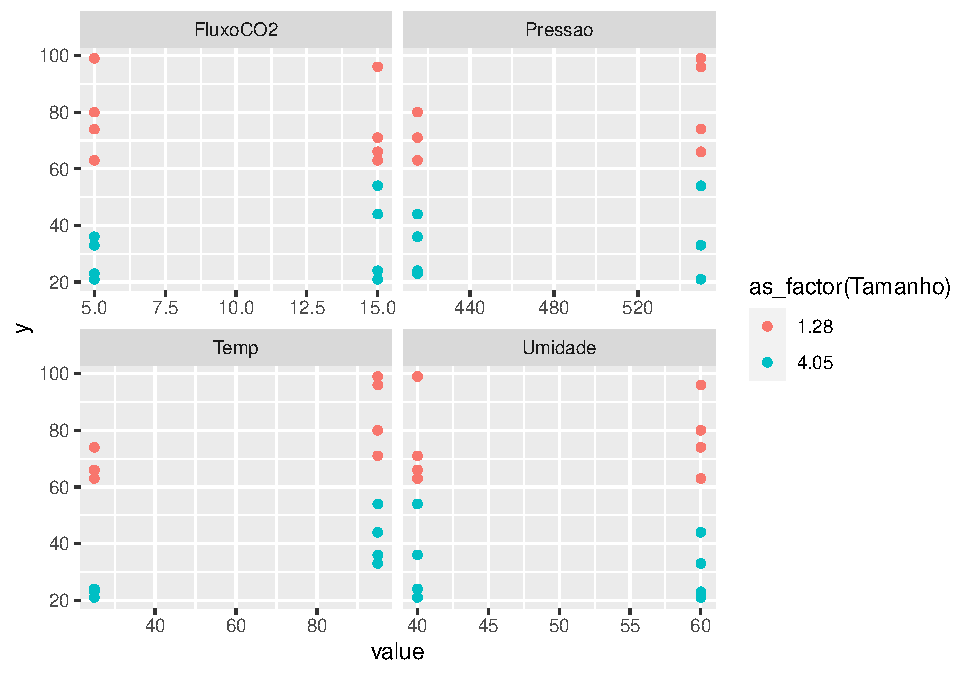
\includegraphics{Exercicio_2_SME0820_Grupo03_files/figure-latex/unnamed-chunk-11-1.pdf}

Interpretando os gráficos acima, podemos observar no histograma que a
distribuição - embora majoritariamente centralizada - ocorre de forma
irregular. No gráfico de dispersão podemos constatar certa normalidade
dos valores, que possuem uma aproximação evidente dos quantis teóricos.
Como estamos fazendo suposições a partir de uma análise interpretativa,
podemos utilizar do teste de Shapiro-Wilk para verificá-las, como segue
abaixo:

\begin{Shaded}
\begin{Highlighting}[]
\FunctionTok{pander}\NormalTok{(}\FunctionTok{shapiro.test}\NormalTok{(res), }\AttributeTok{style=}\StringTok{\textquotesingle{}rmarkdown\textquotesingle{}}\NormalTok{,}
       \AttributeTok{caption =} \StringTok{"Teste de normalidade Shapiro{-}Wilk para os resíduos"}\NormalTok{)}
\end{Highlighting}
\end{Shaded}

\begin{longtable}[]{@{}cc@{}}
\caption{Teste de normalidade Shapiro-Wilk para os resíduos Se
considerarmos a significância como sendo 97\% - como referenciado em
materiais anteriores -, teremos que nosso modelo segue a distribuição
normal, visto que obtivemos um resultado de 0.2733 no teste de
Shapiro-Wilk. Ou seja, não é um valor alto suficiente para rejeitar a
hipótese nula de normalidade dos dados.}\tabularnewline
\toprule
Test statistic & P value \\
\midrule
\endfirsthead
\toprule
Test statistic & P value \\
\midrule
\endhead
0.9544 & 0.2733 \\
\bottomrule
\end{longtable}

Além disso, para determinar matematicamente se existe uma relação linear
entre a variável resposta \(\boldsymbol{Y}\) e qualquer as outras
covariáveis \(\boldsymbol{X}_1,\ldots,\boldsymbol{X}_k\), é possível
utilizar o teste \textbf{ANOVA}. Nele, queremos testar:

\textbf{\(H_0\)}: Nenhuma das variáveis contribui significativamente ao
modelo, versus:

\textbf{\(H_a\)}: Pelo menos uma das covariáveis contribui
significativamente ao modelo.

Tabela \emph{ANOVA}:

\begin{longtable}[]{@{}ccccc@{}}
\caption{Tabela ANOVA}\tabularnewline
\toprule
\textbf{F.V.} & \textbf{G.L} & \textbf{S.Q.} & \textbf{Q.M.} &
\textbf{F} \\
\midrule
\endfirsthead
\toprule
\textbf{F.V.} & \textbf{G.L} & \textbf{S.Q.} & \textbf{Q.M.} &
\textbf{F} \\
\midrule
\endhead
\textbf{Regressão} & \(k\) & \(SQ_{reg}\) & \(QMreg=\dfrac{SQreg}{k}\) &
\(F=\dfrac{QMreg}{QMres}\) \\
\textbf{Resíduo} & \(n-p\) & \(SQ_{res}\) & \(QMres=\dfrac{SQres}{n-p}\)
& \\
\textbf{Total} & \(n-1\) & \(SQ_{total}\) & \(QM_{Total}\) & \\
\bottomrule
\end{longtable}

\begin{Shaded}
\begin{Highlighting}[]
\CommentTok{\# Soma dos quadrados dos residuos  }
\NormalTok{(SQRes }\OtherTok{\textless{}{-}} \FunctionTok{t}\NormalTok{(Y}\SpecialCharTok{{-}}\NormalTok{Y\_est)}\SpecialCharTok{\%*\%}\NormalTok{(Y}\SpecialCharTok{{-}}\NormalTok{Y\_est))}
\end{Highlighting}
\end{Shaded}

\begin{verbatim}
##          [,1]
## [1,] 3222.907
\end{verbatim}

\[SQ_{Reg} = SQ_{Total} - SQ_{Res} = \frac 1n \sum_{i=1}^n y_i^2 - (Y-\hat{Y})^T\cdot(Y-\hat{Y}) =\]
\[\beta^T \cdot X^T \cdot Y - \frac1n (u^T \cdot Y)^2\]

\begin{Shaded}
\begin{Highlighting}[]
\CommentTok{\# Soma dos quadrados totais}
\NormalTok{u }\OtherTok{\textless{}{-}} \FunctionTok{c}\NormalTok{(}\FunctionTok{rep}\NormalTok{(}\DecValTok{1}\NormalTok{,n))}
\NormalTok{(SQTotal }\OtherTok{\textless{}{-}} \FunctionTok{t}\NormalTok{(Y)}\SpecialCharTok{\%*\%}\NormalTok{Y }\SpecialCharTok{{-}}\NormalTok{ ((}\FunctionTok{t}\NormalTok{(u)}\SpecialCharTok{\%*\%}\NormalTok{Y)}\SpecialCharTok{\^{}}\DecValTok{2}\NormalTok{)}\SpecialCharTok{/}\NormalTok{n)}
\end{Highlighting}
\end{Shaded}

\begin{verbatim}
##          [,1]
## [1,] 7870.112
\end{verbatim}

\begin{Shaded}
\begin{Highlighting}[]
\CommentTok{\#Soma dos quadrados da regressao  }
\NormalTok{(SQReg }\OtherTok{\textless{}{-}}\NormalTok{ SQTotal }\SpecialCharTok{{-}}\NormalTok{ SQRes)}
\end{Highlighting}
\end{Shaded}

\begin{verbatim}
##          [,1]
## [1,] 4647.205
\end{verbatim}

\begin{Shaded}
\begin{Highlighting}[]
\CommentTok{\# Calculando a anova}

\NormalTok{k }\OtherTok{\textless{}{-}} \DecValTok{5} 
\NormalTok{p }\OtherTok{\textless{}{-}}\NormalTok{ k}\SpecialCharTok{+}\DecValTok{1}


\NormalTok{gl\_sqreg }\OtherTok{\textless{}{-}}\NormalTok{ k}
\NormalTok{QMReg }\OtherTok{\textless{}{-}}\NormalTok{ SQReg}\SpecialCharTok{/}\NormalTok{gl\_sqreg}

\NormalTok{gl\_sqres }\OtherTok{\textless{}{-}}\NormalTok{ n}\SpecialCharTok{{-}}\NormalTok{p}
\NormalTok{QMRes }\OtherTok{\textless{}{-}}\NormalTok{ SQRes}\SpecialCharTok{/}\NormalTok{gl\_sqres}

\NormalTok{gl\_sqtotal }\OtherTok{\textless{}{-}}\NormalTok{ n}\DecValTok{{-}1}
\end{Highlighting}
\end{Shaded}

\begin{Shaded}
\begin{Highlighting}[]
\CommentTok{\#calculando a estatistica F}
\NormalTok{(F\_0 }\OtherTok{\textless{}{-}}\NormalTok{ QMReg}\SpecialCharTok{/}\NormalTok{QMRes)}
\end{Highlighting}
\end{Shaded}

\begin{verbatim}
##          [,1]
## [1,] 6.056104
\end{verbatim}

\begin{Shaded}
\begin{Highlighting}[]
\NormalTok{(QMTotal }\OtherTok{\textless{}{-}}\NormalTok{ QMRes }\SpecialCharTok{+}\NormalTok{ QMReg)}
\end{Highlighting}
\end{Shaded}

\begin{verbatim}
##          [,1]
## [1,] 1082.913
\end{verbatim}

Como nosso estimador \(F \sim F(k,\ n - k - 1)\), podemos obter os
quantis com o auxílio do R, assumindo \(\alpha = 0.03\) - a partir de
instruções fornecidas em trabalhos anteriores:

\begin{Shaded}
\begin{Highlighting}[]
\NormalTok{alpha }\OtherTok{\textless{}{-}} \FloatTok{0.03}
\NormalTok{(RR }\OtherTok{\textless{}{-}} \FunctionTok{qf}\NormalTok{(alpha, }\AttributeTok{df1 =}\NormalTok{ k, }\AttributeTok{df2 =}\NormalTok{ n }\SpecialCharTok{{-}}\NormalTok{ k }\SpecialCharTok{{-}}\DecValTok{1}\NormalTok{, }\AttributeTok{lower.tail =}\NormalTok{ F) )}
\end{Highlighting}
\end{Shaded}

\begin{verbatim}
## [1] 3.098817
\end{verbatim}

Rejeitamos \(H_0\) se \(F_0 > F_{crit}\), sendo \(F_{crit}\) o quantil
teórico da distribuição F com \(k\) e \(n-p\) graus de liberdade.

\begin{Shaded}
\begin{Highlighting}[]
\ControlFlowTok{if}\NormalTok{(RR }\SpecialCharTok{\textless{}}\NormalTok{ F\_0)\{}
  \FunctionTok{cat}\NormalTok{(}\StringTok{"Rejeita{-}se H0"}\NormalTok{)}
\NormalTok{\}}
\end{Highlighting}
\end{Shaded}

\begin{verbatim}
## Rejeita-se H0
\end{verbatim}

Dessa forma, podemos concluir com 97\% de confiança que pelo menos uma
das variáveis contribui significativamente ao modelo.

\hypertarget{verificando-a-importancia-do-subconjunto-com-x3-x4-e-x5.}{%
\section{Verificando a importancia do subconjunto com x3, x4 e
x5.}\label{verificando-a-importancia-do-subconjunto-com-x3-x4-e-x5.}}

\hypertarget{sob-h_0-ux3b2_2-0-vs-sob-h_1-ux3b2_2-neq-0}{%
\subsection{\texorpdfstring{Sob \(H_0 : β_2 = 0\) VS sob
\(H_1 : β_2 \neq 0:\)}{Sob H\_0 : β\_2 = 0 VS sob H\_1 : β\_2 \textbackslash neq 0:}}\label{sob-h_0-ux3b2_2-0-vs-sob-h_1-ux3b2_2-neq-0}}

Soma de quadrados extra devido a \(x_3\),\(x_4\) e \(x_5\):

\(SQ_{reg}(\beta_3,\beta_4,\beta_5|\beta_0,\beta_1,\beta_2) = SQ_{reg}(\beta_0,\beta_1,\beta_2,\beta_3,\beta_4,\beta_5) - SQ_{reg}(\beta_0,\beta_1,\beta_2)\)
(Não corrigida)

\(SQ_{reg}(\beta_3,\beta_4,\beta_5|\beta_0,\beta_1,\beta_2) = SQ_{reg}(\beta_1,\beta_2,\beta_3,\beta_4,\beta_5|\beta_0) - SQ_{reg}(\beta_1|\beta_0) - SQ_{reg}(\beta_2|\beta_1, \beta_0) - SQ_{reg}(\beta_3|\beta_2,\beta_1,\beta_0)- SQ_{reg}(\beta_4|\beta_3,\beta_2,\beta_1,\beta_0) - SQ_{reg}(\beta_5|\beta_4,\beta_3,\beta_2,\beta_1,\beta_0)\)
(Corrigida)

Temos que:

\(SQ_{reg}(\beta_0,\beta_1,\beta_2) = SQ_{reg}(\beta) = \widehat{\beta}^T X^T \boldsymbol{y}\)

\begin{Shaded}
\begin{Highlighting}[]
\NormalTok{SQReg\_r }\OtherTok{\textless{}{-}}\NormalTok{ (}\FunctionTok{t}\NormalTok{(betas)}\SpecialCharTok{\%*\%}\FunctionTok{t}\NormalTok{(X)}\SpecialCharTok{\%*\%}\NormalTok{Y)}
\NormalTok{SQReg\_r}
\end{Highlighting}
\end{Shaded}

\begin{verbatim}
##          [,1]
## [1,] 21160.17
\end{verbatim}

e

\$SQ\_\{reg\}(\beta\_1,\beta\_2,\beta\_3,\beta\_4,\beta\_5\textbar{}\beta\_0)
= \widehat{\beta}\^{}T X\^{}T \boldsymbol{Y} -
\frac{(I_n^T\boldsymbol{Y})^2}{n} \$

coincide com o valor obtido na tabela ANOVA, sendo este:

\begin{Shaded}
\begin{Highlighting}[]
\NormalTok{SQReg }\CommentTok{\# SQreg encontrado na tabela ANOVA}
\end{Highlighting}
\end{Shaded}

\begin{verbatim}
##          [,1]
## [1,] 4647.205
\end{verbatim}

**

\(Y= \beta_0 + \beta_1X_1 + \beta_2X_2 + \xi\)

Sob \(H_0 : β_2 = 0\):

Considerando o modelo reduzido:

\(Y= \beta_1X_1 + \xi\)

\begin{Shaded}
\begin{Highlighting}[]
\NormalTok{Sxx }\OtherTok{\textless{}{-}} \FunctionTok{sum}\NormalTok{(x1}\SpecialCharTok{\^{}}\DecValTok{2}\NormalTok{) }\SpecialCharTok{{-}}\NormalTok{ n}\SpecialCharTok{*}\NormalTok{(}\FunctionTok{mean}\NormalTok{(x1))}\SpecialCharTok{\^{}}\DecValTok{2}
\NormalTok{Sxy }\OtherTok{\textless{}{-}} \FunctionTok{sum}\NormalTok{(x1}\SpecialCharTok{*}\NormalTok{y) }\SpecialCharTok{{-}}\NormalTok{ n}\SpecialCharTok{*}\NormalTok{(}\FunctionTok{mean}\NormalTok{(x1)}\SpecialCharTok{*}\FunctionTok{mean}\NormalTok{(y))}
\NormalTok{beta\_est\_modredu }\OtherTok{\textless{}{-}}\NormalTok{ Sxy}\SpecialCharTok{/}\NormalTok{Sxx}
\NormalTok{beta\_est\_modredu}
\end{Highlighting}
\end{Shaded}

\begin{verbatim}
## [1] -0.8650001
\end{verbatim}

Agora, tendo o modelo reduzido como sendo:

\(SQ_{reg} = \beta_1Sxy\)

podemos realizar:

\begin{Shaded}
\begin{Highlighting}[]
\NormalTok{SQReg\_modredu }\OtherTok{\textless{}{-}}\NormalTok{ beta\_est\_modredu}\SpecialCharTok{*}\NormalTok{Sxy}
\NormalTok{SQReg\_modredu }\CommentTok{\# 3 G.L. (3 covariáveis no subconjunto)}
\end{Highlighting}
\end{Shaded}

\begin{verbatim}
## [1] 3909.467
\end{verbatim}

\begin{Shaded}
\begin{Highlighting}[]
\NormalTok{gl\_modredu }\OtherTok{\textless{}{-}} \DecValTok{3}
\end{Highlighting}
\end{Shaded}

e, portanto,

\begin{Shaded}
\begin{Highlighting}[]
\NormalTok{SQReg\_teste }\OtherTok{\textless{}{-}}\NormalTok{ SQReg}\SpecialCharTok{{-}}\NormalTok{SQReg\_modredu}
\NormalTok{SQReg\_teste}
\end{Highlighting}
\end{Shaded}

\begin{verbatim}
##          [,1]
## [1,] 737.7382
\end{verbatim}

Este valor representa o aumento na \(SQ_{reg}\) com o acréscimo do
subconjunto no modelo que já possui \(X_1\)

\begin{Shaded}
\begin{Highlighting}[]
\NormalTok{QMReg\_modredus }\OtherTok{\textless{}{-}}\NormalTok{ (SQReg\_teste}\SpecialCharTok{/}\NormalTok{gl\_modredu)}
\NormalTok{F\_testeparcial }\OtherTok{\textless{}{-}}\NormalTok{ (QMReg\_modredus}\SpecialCharTok{/}\NormalTok{QMRes)}
\NormalTok{F\_testeparcial}
\end{Highlighting}
\end{Shaded}

\begin{verbatim}
##          [,1]
## [1,] 1.602332
\end{verbatim}

\begin{Shaded}
\begin{Highlighting}[]
\NormalTok{alpha }\OtherTok{\textless{}{-}} \FloatTok{0.03}
\NormalTok{RR }\OtherTok{\textless{}{-}} \FunctionTok{qf}\NormalTok{(alpha, }\AttributeTok{df1 =}\NormalTok{ gl\_modredu, }\AttributeTok{df2 =}\NormalTok{ n }\SpecialCharTok{{-}}\NormalTok{ gl\_modredu }\SpecialCharTok{{-}}\DecValTok{1}\NormalTok{, }\AttributeTok{lower.tail =}\NormalTok{ F)}
\NormalTok{RR}
\end{Highlighting}
\end{Shaded}

\begin{verbatim}
## [1] 3.556927
\end{verbatim}

\begin{Shaded}
\begin{Highlighting}[]
\ControlFlowTok{if}\NormalTok{(RR }\SpecialCharTok{\textless{}}\NormalTok{ F\_testeparcial)\{}
 \FunctionTok{cat}\NormalTok{(}\StringTok{"Rejeita{-}se H0"}\NormalTok{)}
\NormalTok{\}}
\end{Highlighting}
\end{Shaded}


\end{document}
